\subsection{Road Generation}
The fundamental infrastructure of a city is the road network and as such, it was important to get this right early on in the development of the city generator.
The application needed a method that was both flexible and also offered realistic-looking results.
To generate the road network for the city, a RoadGenerator class was implemented which takes the terrain and the population map as inputs.
These parameters are then used to produce a road network as output, as can be seen in the definition Table~\ref{table:def_roadgen}.

\begin{table}[H]
  \centering
  \begin{tabular}{lllll}
    \textbf{Input} & & \textbf{Function} & & \textbf{Output} \\
    \midrule
    \textit{Terrain, PopulationMap, Markers} & $\rightarrow$ & \textbf{RoadGenerator} & $\rightarrow$ & \textit{RoadNetwork} \\
    \bottomrule
  \end{tabular}

  \caption{Definition of the RoadGenerator which is responsible for generating road networks.}
  \label{table:def_roadgen}
\end{table}
\vspace{-0.4cm}

Two major methods were considered when designing the road generator, one based on a recursive approach where the world is divided into multiple cells with roads placed between these cells.
However, this type of algorithm did not provide realistic-looking results and, while being quite flexible, was overly complex for creating a good road network that mimics reality.

Instead, the algorithm that was chosen was an \textbf{Agent-based} solution that works by simulating road workers, which will be referred to as Agents, whose only goal is walking around the world depending on certain strategies and creating roads.
Agents could also decide to branch into multiple, new Agents, creating intersections in the road network.
The goal of this chapter is to describe how this method was used to generate the cities in the application.

Agents themselves do not move on their own, but if given a blueprint to create a specific road, which is referred to as a strategy, they can move around and place roads where it is told to move.
Which strategy to use depends entirely on what the goal of the generation is, but the focus of this project has been to create a flexible base that could be extended to mimics any type of city generation.
As such, the project only includes basic \textbf{Paris} and \textbf{Manhattan} like strategies, and the generation of main roads are different depending on the city strategy.
Paris-like cities have distinct rings within the city boundaries, while Manhattan-like cities generally follow a more organized and grid-like structure.
The generation of the main roads should mimic these characteristics.

Furthermore, Agents can switch strategy mid-generation, be it randomly, or depending on some variables that the Agent has access to.
One example of this might be that if an Agent detects that there is a relatively low population density, it might decide to switch to a village-type strategy that could produce smaller villages with a different layout than cities like Paris or Manhattan.

Strategies can also define the configuration of the Agent, such as step size, how many steps an Agent can take before terminating, and how many times an Agent can branch.
The strategy that the Agent uses is responsible for deciding when an Agent should terminate, except for step count which is handled automatically for all strategies.

The road generator uses the city markers as input to create the initial Agents that will start creating the road network.
Each city type needs its own preset arguments for the Agents, and this was solved by assigning an Agent factory to each city type.
The goal of the Agent factory is determining starting conditions for Agents depending on the city type.


\begin{wrapfigure}[12]{r}{0.4\textwidth}
  \centering
  \raisebox{0pt}[\dimexpr\height-1\baselineskip\relax]{
    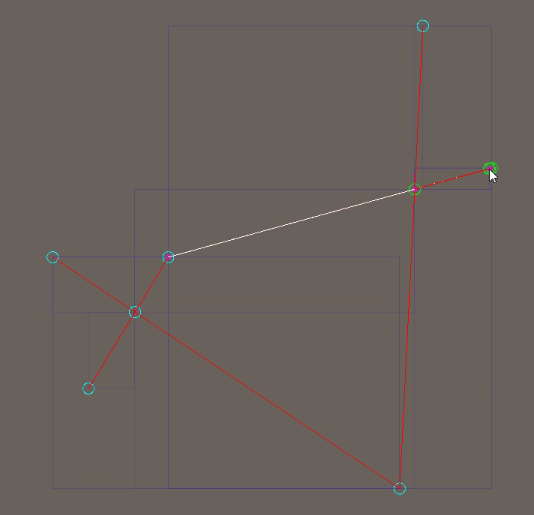
\includegraphics[width=0.36\textwidth]{figure/road_intersection.png}
  }

  \caption{Road intersection and R-Tree bounding boxes}

  \label{fig:road_intersection}
\end{wrapfigure}

While Agent strategies handle how the Agent moves around in the world, it is not what decides how the roads should be placed.
When the Agent decides to place a road, it will attempt to find nearby nodes to snap to by searching in multiple ways.
If no nodes to snap to are found, it will create a road between its last position and its new position, and any roads that exist on the path there in between will be combined into an intersection.
Figure~\ref{fig:road_intersection} demonstrates the intersection created after an Agent attempts to cross another road, as well as an optimization technique making use of an R-Tree. %TODO: REFERENCE

The R-Tree is necessary to quickly search for intersecting roads by avoiding to iterate over all nodes in the road network, or else the performance would result in an unusable application.
Each node is placed in the R-Tree with a bounding box that encapsulates each connecting node.
It is the RoadNetwork class that is responsible for handling these cases when nodes are connecting, not the Agents.
When two nodes are connected, the road network will search for nearby nodes that intersect with the bounding box of the new connection, as well as a snap radius which is declared in the Agent configuration.

Furthermore, there are a few cases where it is preferable to not create new nodes for Agents, but rather snap to nearby nodes or network edges.
The algorithm tests for three different cases, visualized in Figure~\ref{fig:road_snap_cases}.
First, the algorithm will search for nodes along the path to the new node, as well as a radius around the node.
The second test attempts to \textit{``extend''} the node further forward, and if it intersects with an edge, it will create an intersection there.
The last test does another intersection test, but instead of extending the node forward, it will project the node to nearby edges and create an intersection there if it is within the snap radius.

\begin{wrapfigure}[13]{r}{0.4\textwidth}
  \centering
  \raisebox{0pt}[\dimexpr\height-1\baselineskip\relax]{
    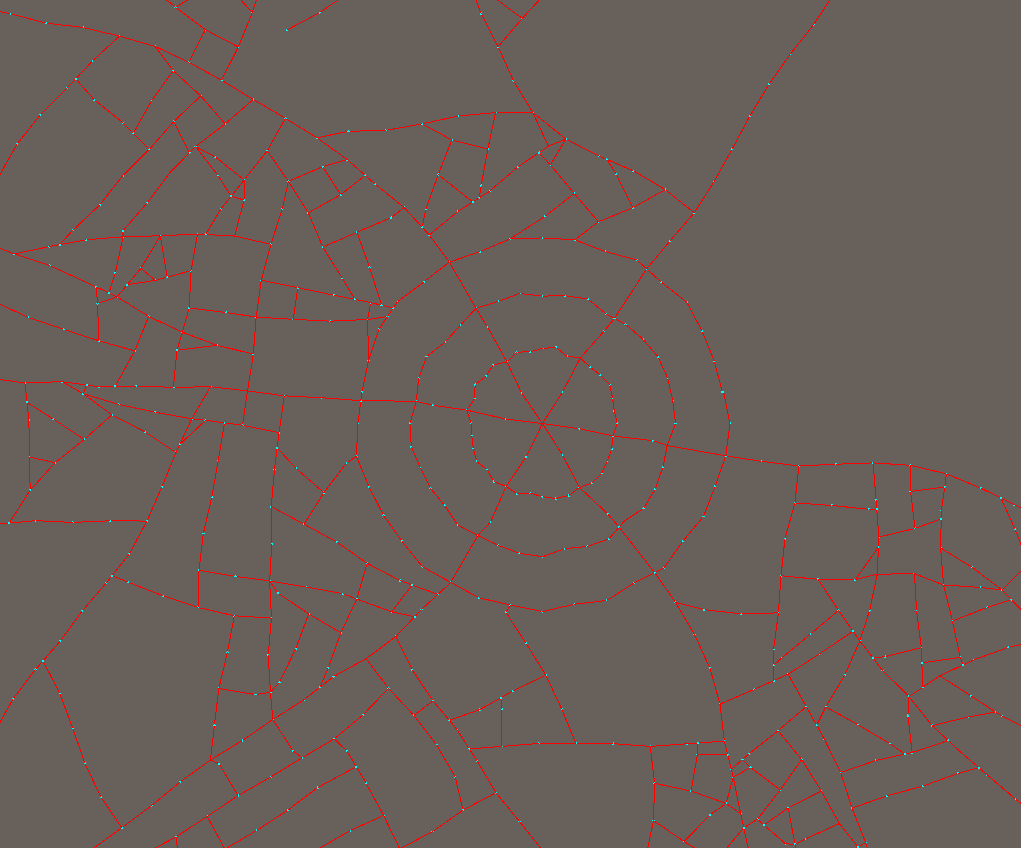
\includegraphics[width=0.36\textwidth]{figure/road_network_paris.png}
  }
  \caption{Example of agent strategy building a Paris-like city shape.}

  \label{fig:road_network_paris}
\end{wrapfigure}

For example, in Figure~\ref{fig:road_network_paris}, the road generator started by creating a ParisAgentFactory, which takes the city position and radius as input, and spawns multiple Agents depending on random variables within the bounds of the input.
The Agents are also given a Paris-like strategy, which instructs the Agents to generate rings around the city center as well as main roads extending outwards.
This particular strategy was configured to have a very aggressive branching, which in turn produces lots of intersections.

So far, the generation of main roads within city bounds has been described, but the world also includes highways that connect multiple cities together.
The goal of highway strategies is instructing Agents to generally move towards higher population areas.
When a suitable strategy is implemented that accomplishes this, other strategies can make use of the ability to switch Agent strategies mid-iteration.

The Paris and Manhattan strategies that were used in the project will switch the Agent strategy to a highway one once the Agent steps outside the boundaries of the city.
This results in Agents that had a tendency to walk towards higher populated areas in the world after it has left the outskirts of the city.
See Figure~\ref{fig:road_highways}.

\begin{figure}[H]
  \centering

  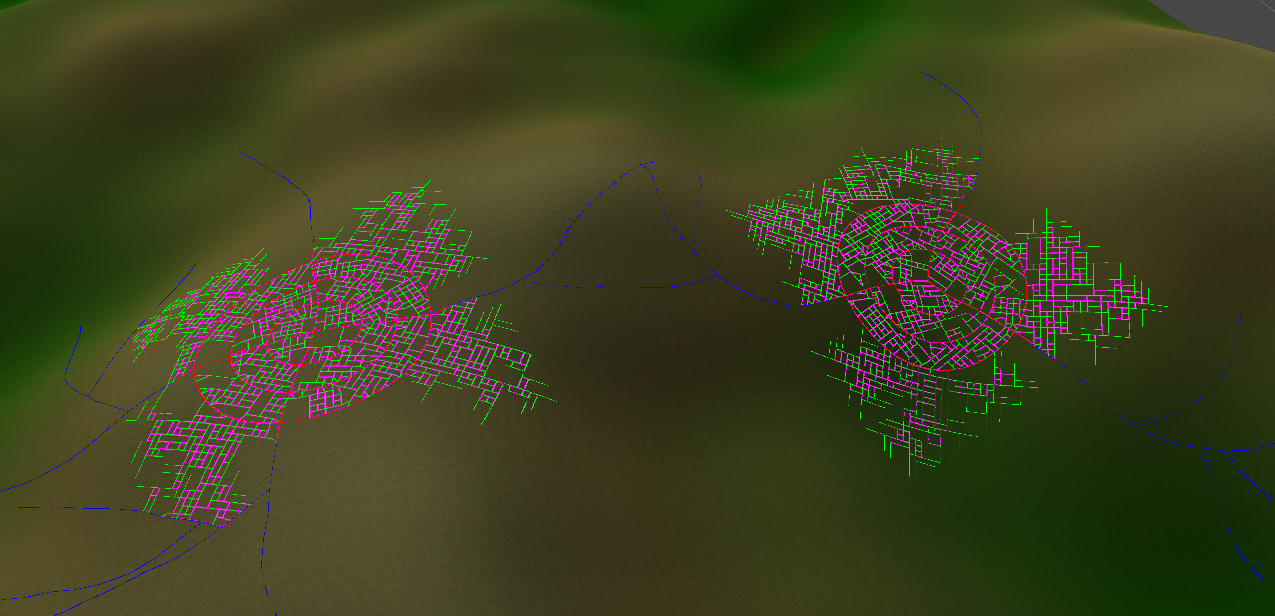
\includegraphics[width=0.8\textwidth]{figure/road_highways.png}
  \caption{Highways created outside the bounds of the city (blue lines), as well as streets (green) with blocks (purple).}

  \label{fig:road_highways}
\end{figure}

The highway strategies that were implemented into the project had a lower probability of branching than other strategies, which produces roads that were longer with fewer exits.
The group aimed to produce highways that mimic the structure of highways in the real world, which this logic usually did.
